\subsection{Atribuição dos referenciais e das variáveis generalizadas}
\label{sec:referenciais_variaveisGeneralizadas}

Foi utilizado referenciais e variáveis generalizadas para realizar a modelagem cinemática e dinâmica do manipulador robótico para então descrever o movimento do MR.
Nesta pesquisa, a convenção de clássica de Denavit--Hartenberg (DH) é utilizada para fixar os referenciais aos elos e representar a transformação geométrica entre eles.

\begin{figure}[ht]
\centering
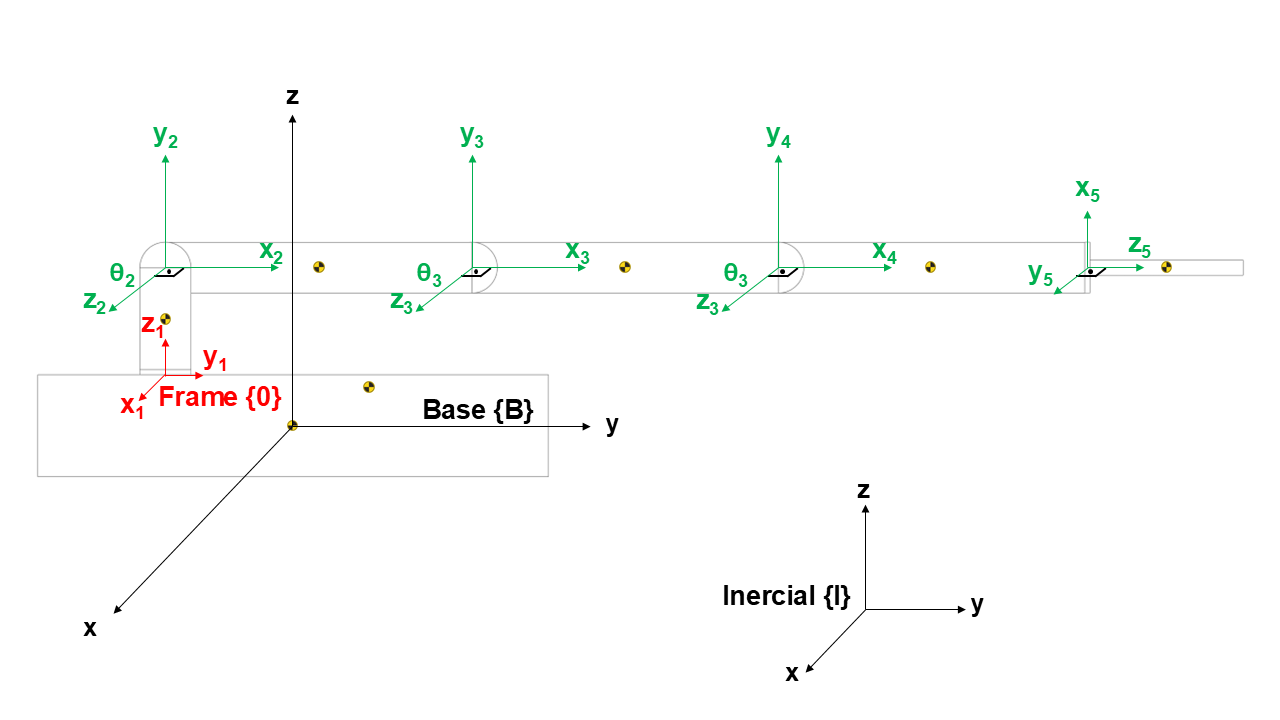
\includegraphics[width=1\textwidth]{2 Formulacao do problema/Imagens/MR Coordenadas locais.png}
\caption{Referencial local do Manipulado Robótico 4R1P acoplado à base.}
\label{fig:frames_MR}
\end{figure}

O sistema de coordenadas inercial $\{I\}$ é utilizado como referência absoluta, enquanto que o referencial da base $\{B\}$ tem sua origem no centro de massa da base e os seus eixos estão alinhados conforme a orientação do corpo, além disso, o referencial $\{0\}$ está na base do primeiro elo do MR.
Os referenciais locais $\{i\}$ ($i=1,\dots,5$) são fixados em cada elo do manipulador, conforme as atribuições de DH:

\begin{enumerate}[label=(\roman*)]
    \item o eixo $Z_i$ coincide com o eixo de rotação (ou de deslizamento) da junta $i$;
    \item o eixo $X_i$ é definido como perpendicular comum entre $Z_i$ e $Z_{i+1}$ e aponta de $Z_i$ para $Z_{i+1}$;
    \item o eixo $Y_i$ completa o sistema dextrogiro.
\end{enumerate}

A posição e a orientação de cada elo em relação ao anterior são expressas pela matriz de transformação homogênea
${}^{i-1}A_i$, expressa por:

\begin{equation}
\label{eq:transformacao_DH}
{}^{i-1} A_i =
\begin{bmatrix}
\cos\theta_i & -\sin\theta_i\cos\alpha_{i-1} & \sin\theta_i\sin\alpha_{i-1} & a_{i-1}\cos\theta_i \\[4pt]
\sin\theta_i & \cos\theta_i\cos\alpha_{i-1} & -\cos\theta_i\sin\alpha_{i-1} & a_{i-1}\sin\theta_i \\[4pt]
0 & \sin\alpha_{i-1} & \cos\alpha_{i-1} & d_i \\[4pt]
0 & 0 & 0 & 1
\end{bmatrix}.
\end{equation}

Faz-se o produto sucessivo dessa matriz para obter a transformação global entre a base e o efetuador $\{E\}$:

\begin{equation}
\label{eq:transformacao_total}
{}^{B} T_{E}
=
{}^{B} T_1\,
{}^{1} T_2\,
{}^{2} T_3\,
{}^{3} T_4\,
{}^{4} T_5,
\end{equation}

sendo que ${}^{B} T_{E}$ descreve a posição e a orientação do efetuador em relação à base.
O estado generalizado do sistema acoplado base--manipulador, é definido pelo o vetor:

\begin{equation}
\label{eq:vetor_q}
\vec{q} =
\begin{bmatrix}
\vec{r}_B \\[4pt]
\vec{\eta}_B \\[4pt]
\vec{\theta}
\end{bmatrix},
\end{equation}

onde:
\begin{itemize}
    \item $\vec{r}_B$ é a posição do centro de massa da base no referencial inercial $\{I\}$;
    \item $\vec{\eta}_B$ descreve a atitude da base e pode ser expressa tanto por ângulos de Euler como por um quaternion unitário $q_B$;
    \item $\vec{\theta} = [\theta_1,\theta_2,\theta_3,\theta_4,d_5]^T$ são as variáveis articulares do manipulador robótico 4R1P.
\end{itemize}

Para relacionar as velocidades lineares e as velocidades angulares dos elos consecutivos utiliza-se a equação diferencial das transformações homogêneas.
Seja ${}^{i-1} \vec{\omega}_i$ a velocidade angular do elo $i$ em relação ao elo anterior $i-1$, e seja ${}^{i-1}\,\vec{v}_i$ a velocidade linear do ponto de origem de $\{i\}$; então:

\begin{equation}
\label{eq:relacao_velocidades}
{}^{i} \vec{v}_i
=
{}^{i}R_{i-1} \left( {}^{i-1} \vec{v}_{i-1} + {}^{i-1} \vec{\omega}_{i-1} \times {}^{i-1} \vec{r}_{i-1,i} \right),
\end{equation}

onde ${}^{i}R_{i-1}$ é a matriz de rotação entre os referenciais e ${}^{i-1} \vec{r}_{i-1,i}$ é o vetor de posição do referencial $\{i\}$ em relação ao anterior $\{i-1\}$.